Before starting to establish a whole 3D mapping, a more simple case can be studied first and it will be shown, in this section, how to determine the distance to only one point. Indeed, the distance between the camera and a point of the target can be easily determined thanks to a little bit of trigonometry.

The context of this case is simple, the camera is recording images of the target while the artificial light source is projecting a point one the last one (see figure \ref{fig:schema1D}).

\begin{figure}[h]
  %\centering
  \centerline{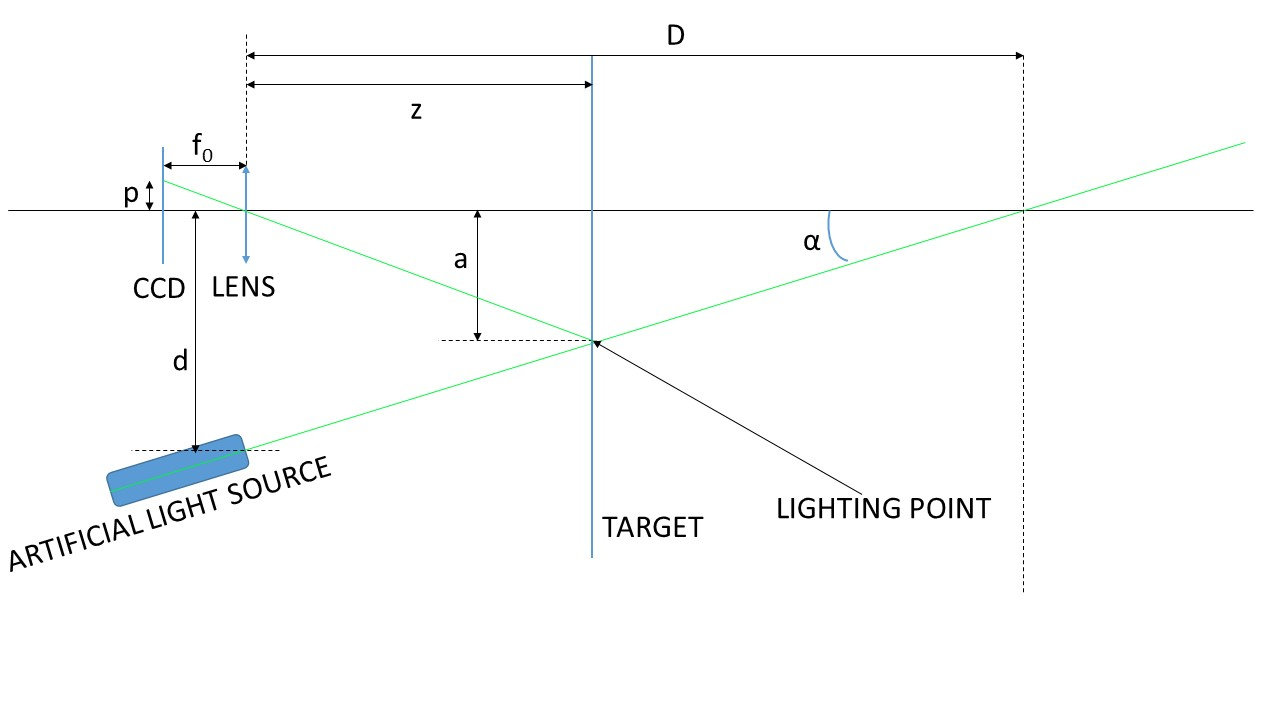
\includegraphics[scale=0.5]{fig/schema1D.jpg}}
  \caption{schema of the camera recording images of the target on which there is a lighting point from the artificial light source}
  \label{fig:schema1D}
\end{figure}

According to the figure \ref{fig:schema1D}, 
\begin{itemize}
\item \textbf{z} is the distance to determine.
\item $\bm{\alpha}$ is the angle between the focal axis of the camera and the focal axis of the light source.
\item \textbf{a} is the distance between the focal axis of the camera and the lighting point.
\item \textbf{D} is the distance between the camera and the lighting point when this one is on the focal axis of the camera.
\item \textbf{d} is the distance between the camera and the light source
\item \textbf{p} is the distance between the focal axis and the image of the lighting point on the CCD
\end{itemize}
Thus, we have

\begin{equation*}
	d=D-\frac{a}{\tan \alpha}
\label{eq:formule_1D}
\end{equation*}


However, $\bm{\alpha}$, \textbf{a} and \textbf{D} are not known yet, that is why a calibration phase is needed (see Figure \ref{fig:calibration}). The first parameter, $\bm{\alpha}$, is determined during the installation of the light source and the camera on the rover. Then, during the calibration, two steps can be identified. During the first one, a target is positioned such as the lighting point is on the center of the image recorded by the camera. Thus, \textbf{D} can be measured. During the second step, a target is positioned such as the lighting point is right on side (left or right) of the image recorded by the camera (see Figure \ref{fig:calibration}). Therefore, $a_0$ can be measured and we have

\begin{equation*}
	\frac{a_0}{p_0} = \frac{z_0}{f_0} \qquad \text{and} \qquad \frac{a}{p} = \frac{z}{f_0}
\end{equation*}

Thus, we have 

\begin{equation*}
	a = \frac{pza_0}{p_0z_0}
\end{equation*}

And finally, 

\begin{equation*}
	z = \frac{Dp_0z_0\tan\alpha}{p_0z_0\tan\alpha+pa_0}
\end{equation*}

The distance $p$ and $p_0$ can be determined using the pixel size $P_{size}$ such as

\begin{equation*}
	p = P_{pixels}P_{size}
\end{equation*}

but the pixel size $P_{size}$ can be simplified and the final formula is

\begin{equation*}
z = \frac{Dp_{pixels\_0}z_0\tan\alpha}{p_{pixels\_0}z_0\tan\alpha+p_{pixels}a_0}\end{equation*}


\begin{figure}[H]
  %\centering
  \centerline{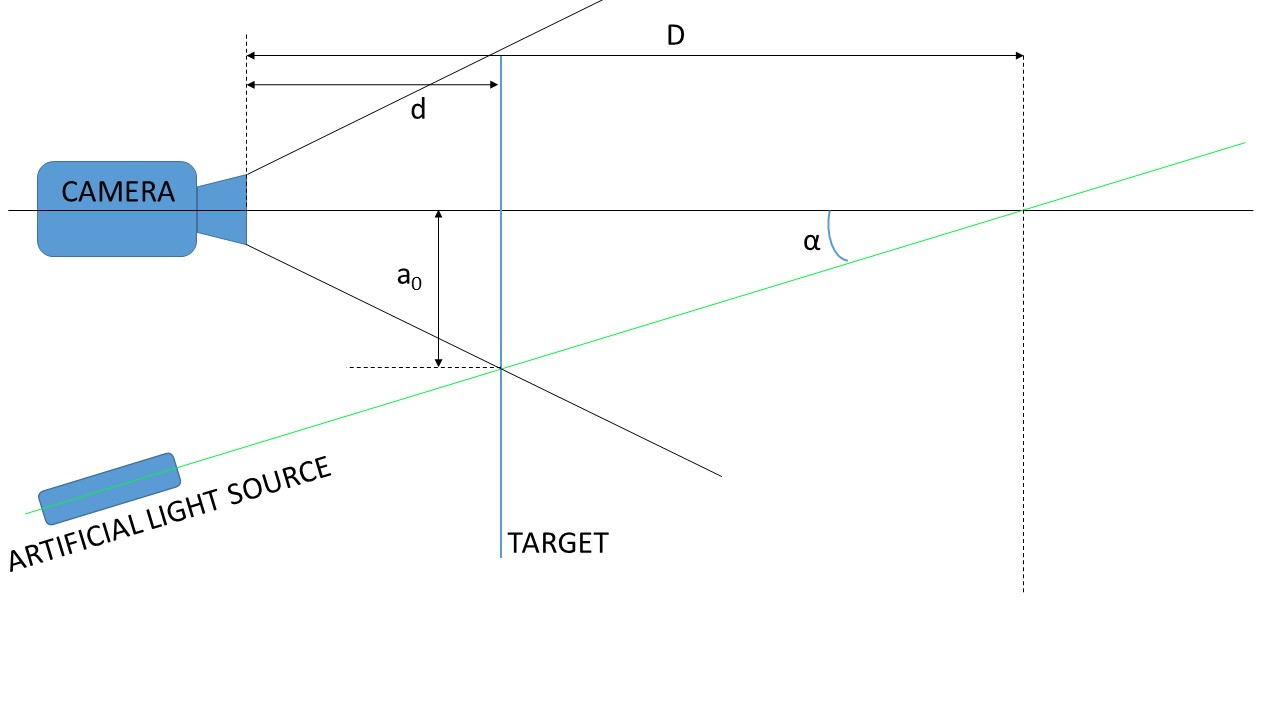
\includegraphics[scale=0.4]{fig/calibration.jpg}}
  \caption{schema of the calibration}
  \label{fig:calibration}
\end{figure}


However, a calculation of the distance camera - target using a simpler calibration can be found thanks to triangulation. Indeed, using the Thales' theorem such as $\frac{z}{f_0} = \frac{a}{p}$ (see Figure \ref{fig:schema1D}), it can be determined that the distance \textbf{z} camera - point on the target is


\begin{equation*}
z = \frac{f_0d}{p+f_0 \tan \alpha}
\end{equation*}

Thus, only the first step of the calibration is needed because only $\bm{\alpha}$ and \textbf{d} need to be determined. $\bm{f_0}$ is a characteristic of the lens and \textbf{p} is determined thanks to the CCD characteristics ($p = p_{pixels} P_{size}$).

\begin{equation}
z = \frac{\frac{f_0}{P_{size}}d}{p_{pixels}+\frac{f_0}{P_{size}} \tan \alpha}
\label{eq:formule1D_2}
\end{equation}